
\chapter*{Chapter \ref{chapter:salval} Supplementary Information}
\chaptermark{Chapter \ref{chapter:salval} Supplementary Information}
\addcontentsline{toc}{chapter}{Chapter \ref{chapter:salval} Supplementary Information}

\vfill

\begin{figure}[h]
    \renewcommand\thefigure{\ref{chapter:salval}.S1}
    \centering
    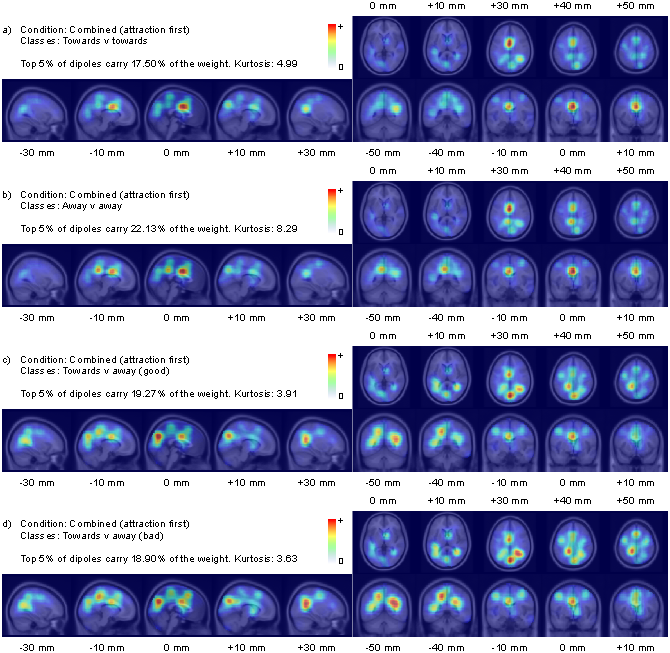
\includegraphics[width=\textwidth]{figures/salval-posfirst-wdd-combined-separate.pdf}
    \caption[Weighted dipole density plots for the two valence-focused and salience focused-classifiers separately, for the attraction-first group.]{Weighted dipole density plots showing the relevance of cortical areas to the two valence-focused and two salience-focused classifiers separately: \emph{a} TvT, \emph{b} AvA, \emph{c} TvT+ and \emph{d} TvT--, all for the attraction-first group.}
    \label{fig:posfirst-wdd-combined-separate}
\end{figure}

\vfill\null\clearpage

\null\vspace{55pt}

\vfill

\begin{figure}[h]
    \renewcommand\thefigure{\ref{chapter:salval}.S2}
    \centering
    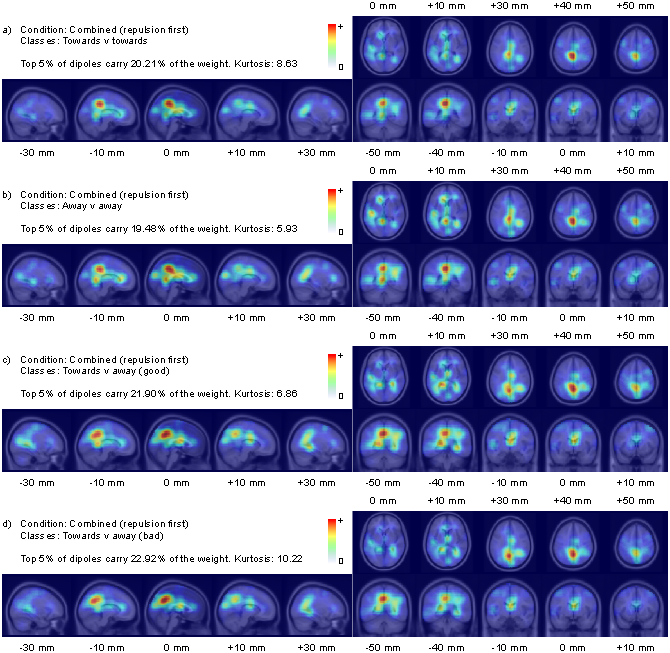
\includegraphics[width=\textwidth]{figures/salval-negfirst-wdd-combined-separate.pdf}
    \caption[Weighted dipole density plots for the two valence-focused and salience focused-classifiers separately, for the repulsion-first group.]{Weighted dipole density plots showing the relevance of cortical areas to the two valence-focused and two salience-focused classifiers separately: \emph{a} TvT, \emph{b} AvA, \emph{c} TvT+ and \emph{d} TvT--, all for the repulsion-first group.}
    \label{fig:negfirst-wdd-combined-separate}
\end{figure}

\vfill\null